%************************************************
\chapter{Docker}\label{ch:docker}
%************************************************
This chapter will present a brief introduction to Docker containers.  Design, develop, test, and document a functional proof-of-concept prototype using Docker containers. This builds on top of topic 1 and should be able to

\begin{itemize}
\item Build docker containers of each service in topic 1
\item Run docker containers locally and on a Raspberry Pi
\item Deploy images to Docker Hub
\end{itemize}


Docker containers allows packaging of software applications with all its dependencies and libraries. It makes it easier to create, deploy and run the applications. The virtual file system  packed in a Docker container can be seen below in figure \ref{fig:filesystem}.

\begin{figure}[bth]
  \centering

      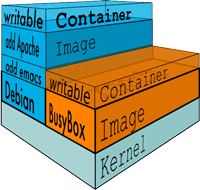
\includegraphics[width=0.4\textwidth]{gfx/what_is_layered_filesystems_sm}
  \caption{Overview of container architecture with complete file system }
  \label{fig:filesystem}
  
\end{figure}




The main purpose of Docker is to ship the whole application with it's whole environment configuration as a single package so that it easily can run on other environments, regardless of any customized settings the particular machine might have.


\begin{figure}[bth]
    \centering
    \subfloat[Vm diagram]{{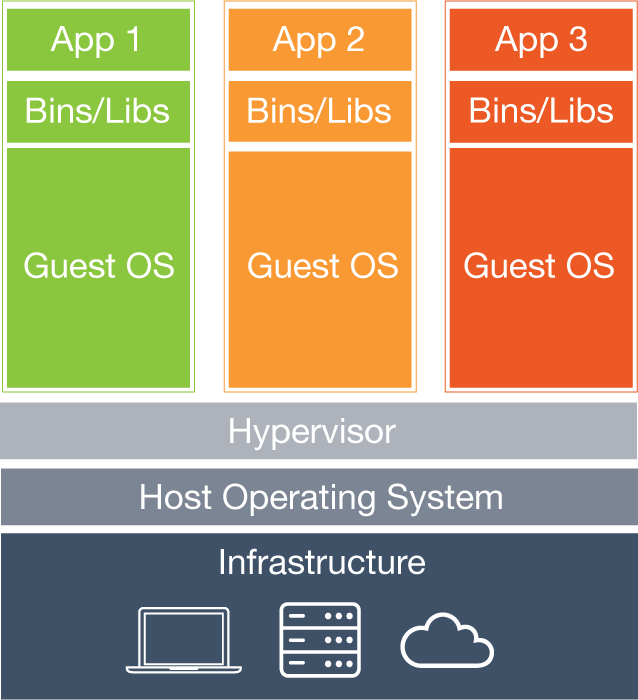
\includegraphics[width=5cm]{gfx/what-is-docker-diagram} }}
    \qquad
    \subfloat[Docker diagram]{{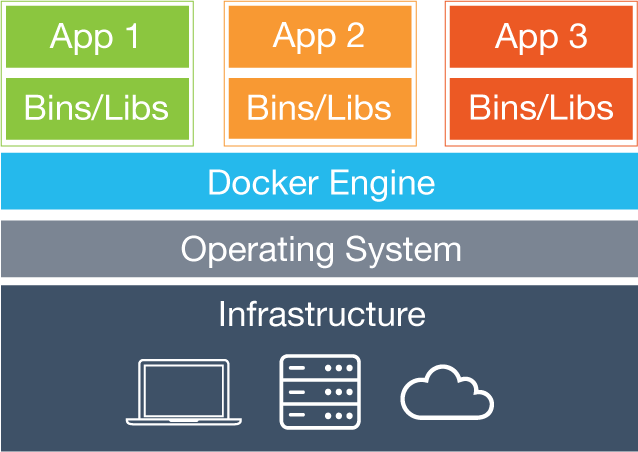
\includegraphics[width=5cm]{gfx/what-is-vm-diagram} }}
    \caption{Docker vs Vm}
    \label{fig:dockervm}
\end{figure}

Docker has resemblance to virtual machines in a way as it can be seen in figure \ref{fig:dockervm}, but Docker allows applications to use the same Linux kernel as the system that they’re running on. By using Docker one can bypass creating virtual machine for every application. 

%An algorithm can be run in docker using any Linux compatible language such as C, Python, Matlab etc. and be compiled using any Linux compatible libraries without causing version or library conflicts with other algorithms.

A docker container can be run at any time with the confidence of that the docker container’s computational environment will be identical. The docker projects remains backwards compatible. 


There are 2 significantly different ways of building Docker containers:

\begin{enumerate}
	\item Interactively
	\item Dockerfile
\end{enumerate} 

Building a container interactively make it possible to install libraries and configure the environment from a shell just like in a typical Linux environment. The modifications can be saved via commits identical to Git, it’s possible to track changes and see the status of modification.\\  

On the other hand Dockerfile builds a container entirely through commands. A Dockerfile identifies a source container to start from (typically a basic Linux installation), then records a series of commands to install libraries and configure the environment. Dockerfiles can also load other Dockerfiles allowing for environment layering and concise organization of various software development projects. Dockerfiles can be versioned using a standard source control versioning tool like Git, allowing revision tracking and archiving of the computational environment.\\

\subsection{PoC of Docker container}
All the services in this project are packed using Docker containers. The Docker containers has all the necessary components and libraries to run a particular service. 

In this project the Dockerfile technique is used to create Docker containers. \cite{Docker2014}

\begin{lstlisting}[frame=single,caption={Dockerfile with command to be carried out},label={{lst:DockerListing}},language=Java]
FROM hypriot/rpi-java
COPY contact-0.0.1-SNAPSHOT.jar /data/
EXPOSE 9003
CMD ["java", "-jar", "contact-0.0.1-SNAPSHOT.jar"]
\end{lstlisting}

The listing \ref{lst:DockerListing} shows a Dockerfile example used to build a Docker-image for Contact service. %The Docker file consists of commands which targets the files placed in the target folder. 

%\begin{lstlisting}[frame=single]
%  COPY /target/Homepage-0.0.1-SNAPSHOT.jar /data/
%\end{lstlisting}
%The command line above specifies that the .jar file should be copied to the container
%
%\begin{lstlisting}[frame=single]
%  EXPOSE 8080
%\end{lstlisting}
%
%The command line above instructs Docker to expose the default Spring Boot port on port 8080. 
%\begin{lstlisting}[frame=single]
%  WORKDIR /data/
%\end{lstlisting}
%
%
%The command line above instructs Docker to change the work directory to where the .jar file is placed. 
%\begin{lstlisting}[frame=single]
%  CMD ["java","-jar","Homepage-0.0.1-SNAPSHOT.jar"]
%  
%\end{lstlisting}
%
%The last command line instructs the container to run the .jar file. 

The \textit{docker build} command does all the heavy-lifting by creating docker image from Dockerfile. This is shown below:

\begin{lstlisting}[frame=single]
$ docker build -t bilalkais/contact:latest
\end{lstlisting}

After building the image the \textit{docker push} command is used to push the image to the Docker-hub repository. Figure \ref{fig:dockerHub} shows a screenshot of three pushed Docker-images.

\begin{figure}[bth]
	\centering
		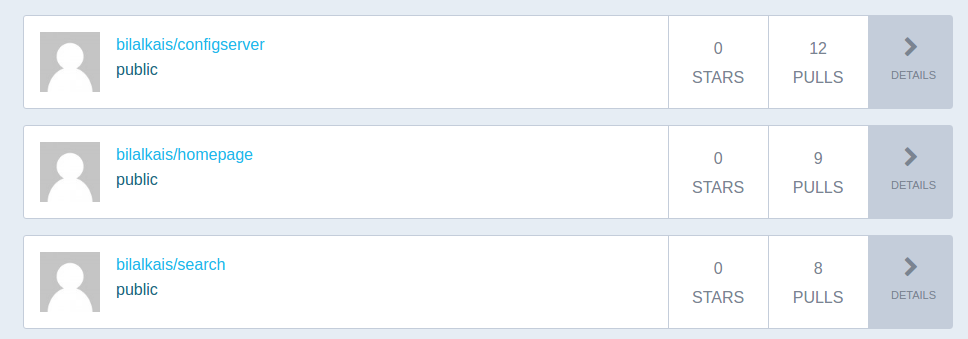
\includegraphics[width=1\textwidth]{gfx/dockerHub}
	\caption{Overview of container architecture with complete file system }
	\label{fig:dockerHub}
\end{figure}

To test the builded Docker-image the \textit{docker run} command is used to run the container using the specified image as shown below:
\begin{lstlisting}[frame=single]
$ docker run --name contact -e AUTOR="bilalkais" -d -P bilalkais/contact
\end{lstlisting}

 %Which is explain in figure \ref{fig:DockerRun}.

%\begin{figure}[bth]
%  \centering
%      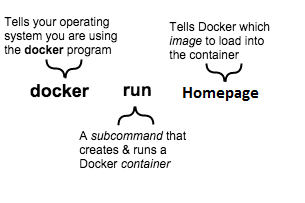
\includegraphics[width=0.5\textwidth]{gfx/container_explainer}
%  \caption{Container explainer}
%  \label{fig:DockerRun}
%\end{figure}


%After running the application in Docker the service then can be accessed using the browser where the IP address is 127.0.0.1 and with the chosen port number.
%
%\begin{lstlisting}
%http:\\localhost:8080
%\end{lstlisting} 
%
%When verifying the service one noticeable thing was that the services was quite slow when they were deployed to the Raspberry Pi, which does make sense. The development computer used for running the the service locally was much faster then the Raspberry Pi. 
%
%The services was pushed to the Docker hub by doing so the Docker checks for the latest version of the application to be run. 
%
%Docker while running provides a lots of information about running Docker containers. 
%
%
%\begin{figure}[bth]
%  \centering
%      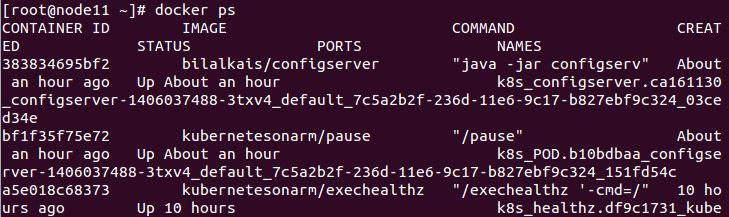
\includegraphics[width=0.5\textwidth]{gfx/DockerPs}
%  \caption{The Docker application running}
%   \label{fig:DockerPs}
%\end{figure}










 